%\documentclass[12pt,letterpaper,margin=0.75in]{article}
%\documentclass[12pt]{article}

\documentclass[12pt, onecolumn]{IEEEtran}

\usepackage[utf8]{inputenc}
\usepackage{amsmath}
\usepackage{amsfonts}
\usepackage{amssymb}
\usepackage{graphicx}
\author{George Engel\\
IC Design Research Laboratory\\
Southern Illinois University Edwardsville\\
}
\usepackage{geometry}

\geometry{
 letterpaper,
% total={8.5in,11in},
 left=1.0in,
 right=1.0in,
 top=1.0in,
 bottom=1.0in,
 }

\usepackage{filecontents}
\usepackage[noadjust]{cite}


\title{Design of a Constant Fraction Discriminator}

\begin{document}

% Insert title

\maketitle

% INTRODUCTION

\section*{Introduction}


A block diagram for the constant fraction discriminator is presented in Figure~\ref{FIG:CFD_BLOCK_DIAGRAM}.
The design presented herein is similar to the discriminator circuit currently being used in our group's HINP4 IC which in turn is based on a design described in xxxx . The design presented in \cite{507173} was executed in 1.2 micron CMOS and boasts timing walk for 5 ns (10 \% - 90 \%) risetime signals over a 40 dB dynamic range (20 mV to 2 V) of less than $\pm$ 150 ps.  The reported jitter was 100 ps with an input level of 20 mV. 


\begin{figure}[htbp!]
	\centering
 	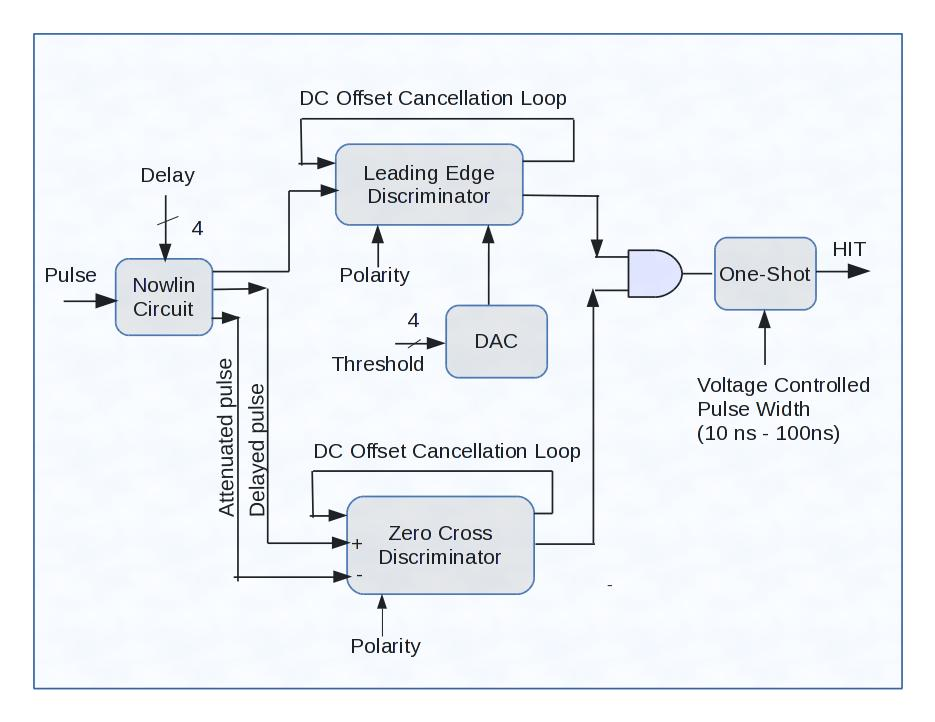
\includegraphics[scale=0.5,keepaspectratio=true]{./images/cfd_block_diagram.jpg} 	
 	\caption{Block diagram of constant fraction discriminator module}
 	\label{FIG:CFD_BLOCK_DIAGRAM}
\end{figure}


The input pulse is assumed to be an exponential, characterized by a rise time constant, $\tau_r$ and a fall time constant, $\tau_f$.  Typically, the ratio $\frac{\tau_f}{\tau_r}$ which we shall call, r, is between 10 and 100. Unless otherwise stated we will assume that this ratio, r, is 100. The input pulse can be modeled using the equation \\

\begin{equation}
x(t) = A \cdot (e^{-\frac{t}{\tau_f}} - e^{-\frac{t}{\tau_r}}).
\end{equation}\\


If the ratio, r, if very large ($>$ 100) then the peak amplitude is approximately A.  For significantly smaller values of r, the peak amplitude can be somewhat smaller than A. For example, for r equal to 10, the peak amplitude is about 70\% of A while for a r value of 100, then it is about 94\% of A.  It is not difficult to prove that the peak amplitude is given by the expression\\

\begin{equation}
Peak Amplitude = A \cdot \left[ e^{-\frac{\tau_{eq}}{\tau_f} \cdot ln(r)} - e^{-\frac{\tau_{eq}}{\tau_r} \cdot ln(r)} \right].
\end{equation}\\


The CFD circuit must support pulses of both positive and negative polarity. The output of the CFD must be a low-jitter, digital pulse of specified duration (50 ns, 100 ns, 200 ns, or 500 ns).  It is critical that the time at which the pulse occurs \textbf{not} depend upon the amplitude, A, of the analog input pulse.  The IC must support analog input pulses with characteristic rise time constants between 2 ns and 192 ns for peak amplitudes in the range of 15 mV to 1.5 V. \\

Moreover, the CFD must exhibit both excellent walk and jitter characteristics.  In order for the time at which the digital one-shot pulse transitions from low-to-high not to be dependent on the input amplitude of the pulse, a "Nowlin" circit is utilized. The "Nowlin" circuit transforms the uni-polar pulse into a bi-polar pulse whose zero-crossing time is independent of pulse amplitude.\\

The leading edge discriminator circuit shown in the Figure~\ref{FIG:CFD_BLOCK_DIAGRAM} consists of a cascade of 3 very high bandwidth but relatively low gain ($\approx 4.5$) differential amplifiers. A "slow" DC offset cancellation loop drives the input referred offset for the cascaded amplifier to the milli-volt level. The amplified (offset-free) output is then compared with a programmable threshold using a continuous-time comparator. The zero cross discriminator circuit shown in the Figure~\ref{FIG:CFD_BLOCK_DIAGRAM} also consists of a cascade of 5 very high bandwidth but relatively low gain ($\approx 4.5$) differential amplifiers. Jut like in the leading-edge preamplifier, a "slow" DC offset cancellation loop in the zero-cross circuit drives the input referred offset for the cascaded amplifier to a very low value but this time to the 100 $\mu V$ level. \\


The output from the leading edge circuit qualifies the output from the zero-cross circuit.  The leading edge comparator transitions \emph{first} followed by the firing of the zero-cross discriminator, thereby accurately marking input pulse arrival time. The ANDing of the zero-cross and leading-edge outputs prevents fallse triggering due to noise. We will now describe each of the blocks shown in the Figure~\ref{FIG:CFD_BLOCK_DIAGRAM} in additional detail. \\

\section*{Design of Nowlin Circuit}

In order to meet our walk and jitter specifications over such a large range of rise times (2 ns to 128 ns), the proposed Nowlin circuit must be highly programmable. We propose both "coarse" and "fine" grain adjustment of the Nowlin circuit.  The coarse grain adjustment is achieved by providing two modes, which we shall refer to as  the "short' and "long" modes.  In the "short" mode the circuit must handle rise time constants in the range from 1 ns to 16 ns (in 1 ns increments) while in "long" mode the propose IC will accommodate risetimes from 12 ns to 192 ns (in 12 ns increments). \\

The fine adjustment is accomplished through the use of a programmable capacitor array.  In other words, 10 - 90 \% ristimes in the range of 2 ns to 420 ns will be supported by the IC. A 4-bit digital code allows the user to select one of 16 capacitor values from 0.5 pF to 8 pF (in 0.5 pF increments), thereby providing the "fine" adjustment.  The circuit for the long mode is presented in Figure~\ref{FIG:NOWLIN_SHORT} while the circuit for the "long" mode is given in Figure~\ref{FIG:NOWLIN_LONG}.\\

\begin{figure}[htbp!]
	\centering
 	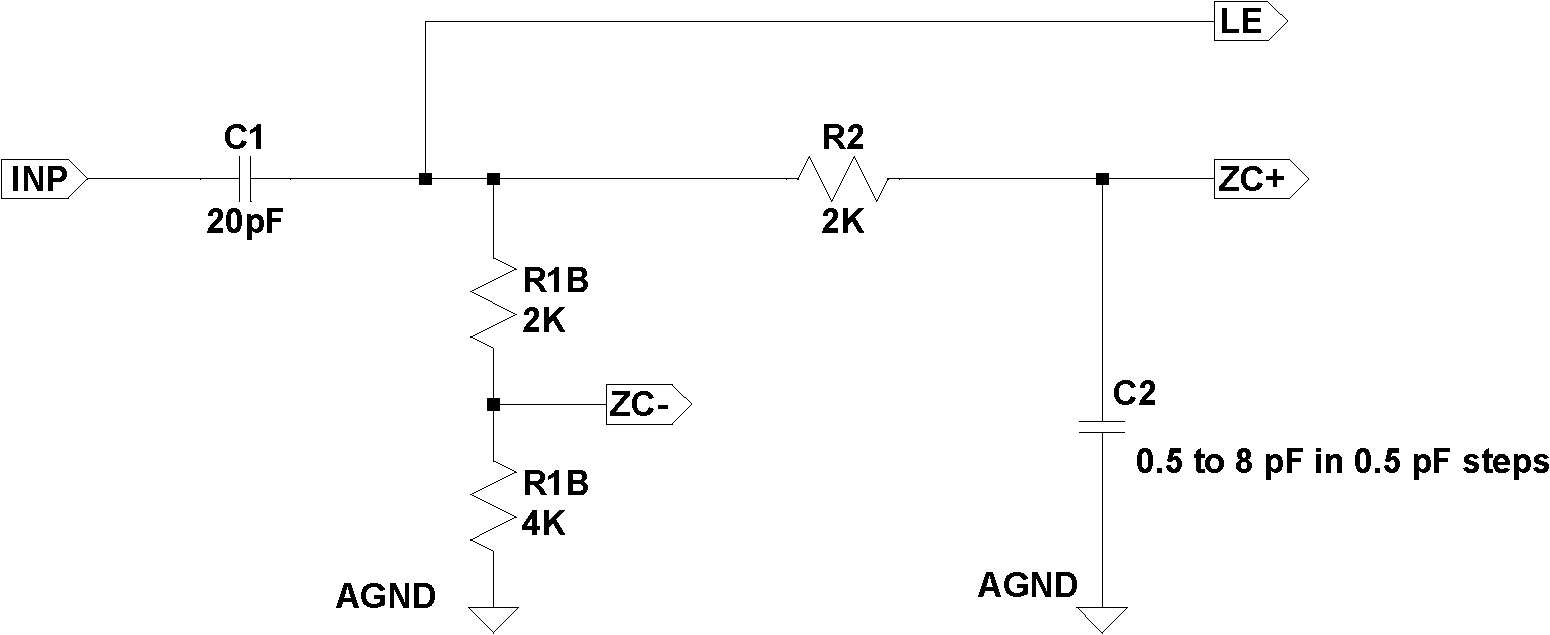
\includegraphics[scale=0.55,keepaspectratio=true]{./images/nowlin_short.pdf} 	
 	\caption{Nowlin circuit to be used in "short" mode.}
 	\label{FIG:NOWLIN_SHORT}
\end{figure}

\begin{figure}[htbp!]
	\centering
 	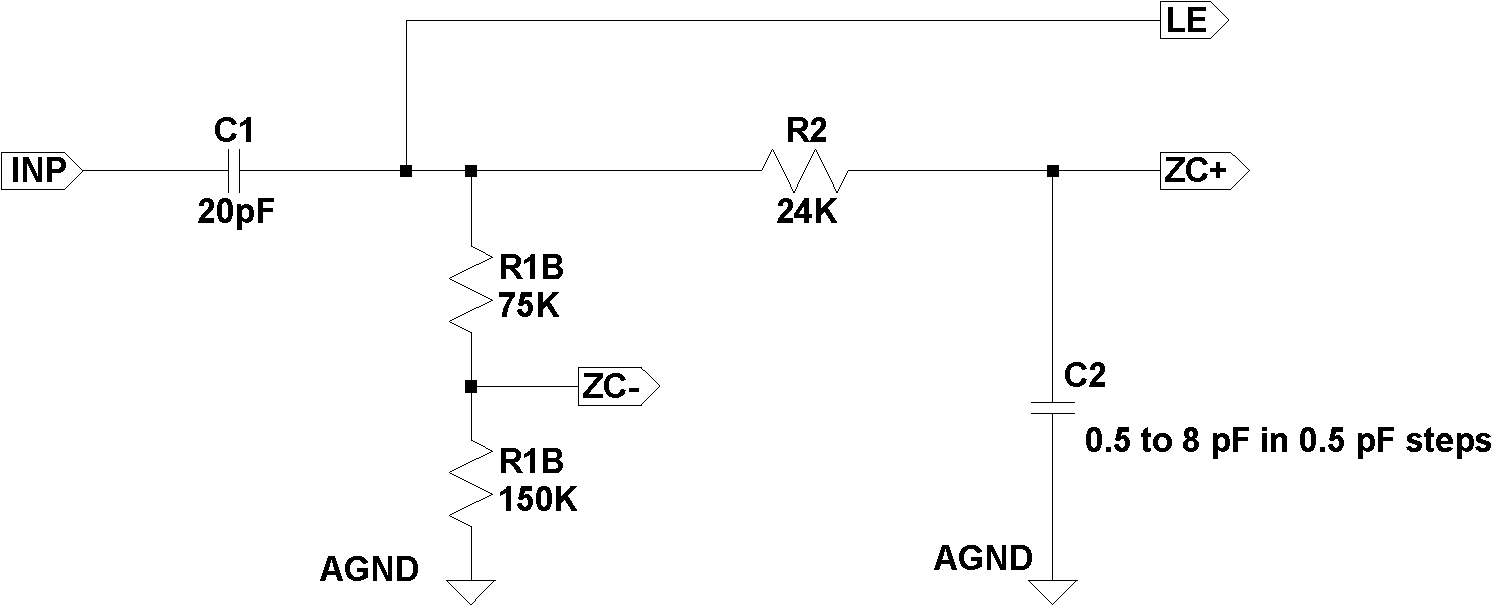
\includegraphics[scale=0.55,keepaspectratio=true]{./images/nowlin_long.pdf} 	
 	\caption{Nowlin circuit to be used in "long" mode.}
 	\label{FIG:NOWLIN_LONG}
\end{figure}


The capacitor, $C_1$, along with resistor, $R_1$, form a highpass filter or what is often referred to as a "fast shaper". The value of $R_1$ is the series combination of resistors $R_{1A}$ and $R_{1B}$. This corresponds to a corner frequency of approximately 1.3 MHz in the "short" mode and about 35 kHz in the "long" time constant mode. \\


The resistor $R_2$ and the programmable capacitor $C_2$ form a delay circuit. The associated time constant, $\tau_n$ = $R_2 \cdot C_2$, is what we shall call the Nowlin delay constant.  The fraction, K = $\frac{R_{1A}}{R_{1A} + R_{1B}}$, helps determine the amount of underdrive.  A "typical" value for K is $\frac{2}{3}$ and that is what we chose to use here. It is important that the comparator in the zero-cross circuit be driven low first and then high since it is the low-high transition that marks the onset of the pulse in an amplitude independent manner. It is important that the comparator underdrive and overdrive be comparable.\\ 


While the input to the Nowlin circuit is an exponential unipolar pulse with amplitude , $\approx A$, and risetime constant, $\tau_r$.  The signal associated with the differential output (\emph{i.e.} difference in voltage on the ZC+ and ZC- nodes) from the Nowlin circuit, however, is a bipolar pulse centered around analog signal ground (or what we will call AGND).  The bipolar signal crosses through zero when the attenuated input signal and the delayed input signal are equal to one another. In other words\\

\begin{equation}
k \cdot A \cdot \left[ 1 - e^{\frac{-t}{\tau_r}} \right] = A \cdot \left[ 1 - e^{\frac{-(t - t_o)}{\tau_r}} \right]
\end{equation}\\

Notice that the amplitude, A, cancels out in the above expression and the time at which this bipolar pulse crosses through zero is independent of pulse amplitude. The delay, $t_o$ is approximately equal to the Nowlin time constant, $\tau_n$ $\approx $ $\tau_r$. This results in a zero-crossing time\\

\begin{equation}
t_z \approx \tau_r \cdot ln \left[ \frac{e - k}{1-k}\right] \approx 1.8 \cdot \tau_r.
\end{equation}

We shall refer to the slope of this signal, when crossing through zero, as the slew rate (SR) given by\\

\begin{equation}
SR \approx \frac{A}{4 \cdot \tau_r}.
\end{equation}


For the minimum pulse amplitude, A, of 15 $mV$ (and r value of 100) and a rise time constant, $\tau_r$, this results in a $SR_{max}$ of 1.7 $\frac{V}{\mu s}$. One can see from Figure~\ref{FIG:NOWLIN_RESPONSE} that it is important that the Nowlin delay constant be matched to the risetime constant. If the Nowlin delay time constant is much too short, we have insufficent underdrive to the comparator to force it to the low state.  If the delay time constant is much too big, then the underdrive is large but the slew rate suffers. Setting the Nowlin delay time constant approximately equal to the rise time constant of the input waveform provides a good compromise between large underdrive and high slew rate.\\

\begin{figure}[htbp!]
	\centering
 	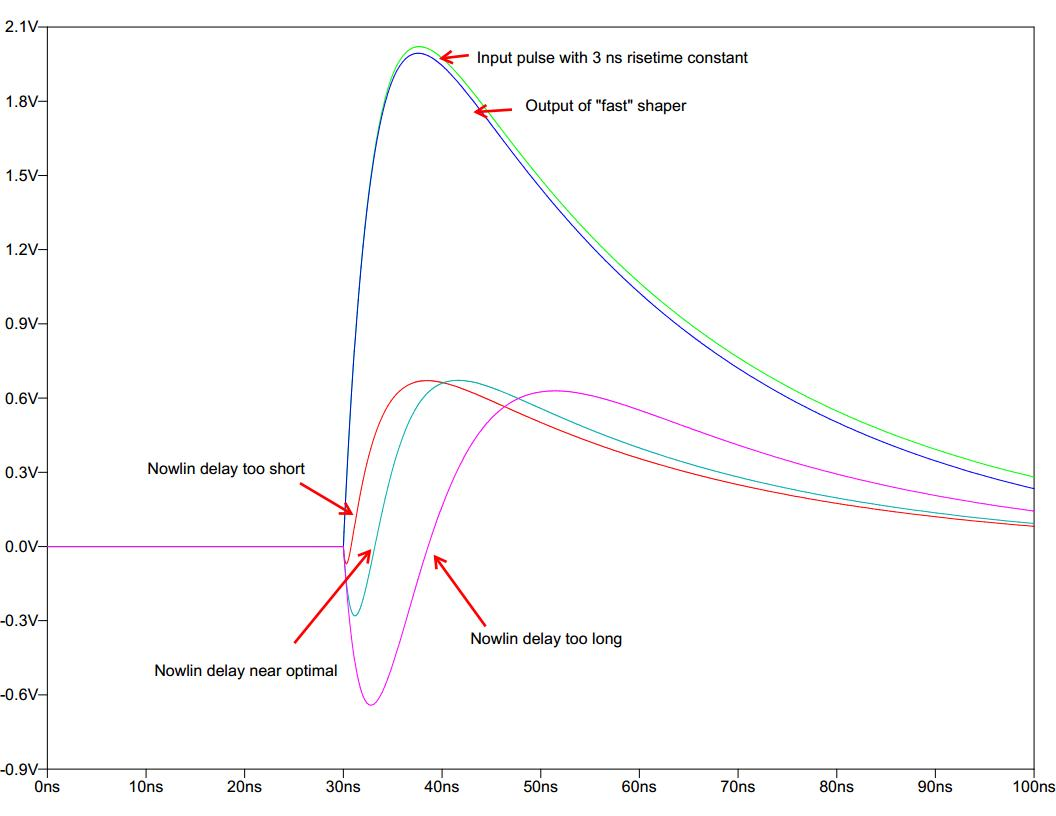
\includegraphics[scale=0.6,keepaspectratio=true]{./images/nowlin_response.jpg} 	
 	\caption{Nowlin circuit response to a signal with rise time constant of 3 ns.}
 	\label{FIG:NOWLIN_RESPONSE}
\end{figure}

\section*{Jitter and Time Walk Analysis}


We analyze jitter first.  Jitter is a consequence of the electronics noise associated with the Nowlin circuit as well as the noise of the \emph{first} differential amplifier in the zero-cross discriminator circuit (where we assume the noise of succeeding stages when referred to the input is negligible).\\


Worst case timing jitter can be estimated by taking the total integrated noise at the input to the zero-cross preamplifier and then dividing by the worst case SR given above.  The noise voltage is due to the thermal noise of the input devices on the first differential amplifier stage, the thermal noise of the gain-setting resistors in that stage, and the thermal noise of the resistors in the Nowlin circuit.  Jitter can be minimized by biasing the input FETs at high current levels and keeping all resistor values small.\\

\begin{equation*}
\sigma_t = \frac{\sigma_v}{SR}
\end{equation*}\\

%\begin{table}[htbp!]
%\begin{center}
%\begin{tabular}{||c | c | c | c||} 
%\hline
%Amplitude (V) & $\sigma_t$ ($\tau_r = 3 ns$) (ps) & $\sigma_t$ ($\tau_r = 15 ns$) (ps) & $\sigma_t$ ($\tau_r = 100 ns$) (ps) \\ [0.5ex] 
%\hline\hline
%1.5 & 1 & 5 & 33\\ 
%\hline
%0.15 & 10 & 50 & 330  \\
%\hline
%0.015 & 100  & 500  & 3300\\ [1ex] 
%\hline
%\end{tabular}
%\end{center}
%\caption{Time jitter as function of pulse amplitude and risetime constant.}
%\label{JitterTable}
%\end{table}


We analyze time walk next.  Time walk is is used to describe systematic variation in the rising edge of the discriminator output signal as a function of pulse height.  If we assume a single-pole response for the analog comparator with a gain-bandwidth-product of $GBW_c$, it is not difficult to show that the variation in propagation delay, $\Delta t_{pd}$, due to input pulse amplitude is \\

\begin{equation*}
\Delta t_{pd} \approx  \sqrt{\frac{V_{DD}}{2 \cdot \pi \cdot GBW_c \cdot G^N \cdot SR_{min}}}
\end{equation*}


where $V_{DD}$ is the supply voltage, G is the gain of a single differential amplifier stage, N is the number of stages, and $SR_{min}$ is  the SR with a pulse amplitude of 15 mV.   Table~\ref{WalkTable} summarizes the expected walk performance (over the dynamic range of 15 mV - 1.5 V) for three representative risetime constants.\\


In reality, the time walk may increase at low amplitudes because of residual offset.  Ultimately, how well the discriminator performs at low amplitude will depend on the effectiveness of the dynamic offset cancellation loop, shown in Fig.~\ref{BlockDiagram}.  It can be shown that residual offset alters the time at which one crosses zero as given by\\

\begin{equation*}
\Delta t_{cross} \approx \tau_r \cdot \left[ \frac{V_{os}}{(1-k) \cdot A} \right]
\end{equation*}


where $V_{os}$ is the residual input referred offset and A is the amplitude of the input pulse. It is important that the residual offset be driven to the sub-mV level.  The "slow" DC offset cancellation loop has to be "slow" enough so as not to interfere with the pulse as it passes through the zero-cross discriminator but yet fast enough so that pulse repetition rates as high as 1 kHz can be accommodated.  This will require significant design effort but is certainly feasible, as demonstrated in \cite{507173}. The wide range of pulse risetime constants we wish to support makes this problem more difficult but not impossible.\\

\begin{table}[htbp!]
\begin{center}
\begin{tabular}{||c | c||} 
\hline
$\tau_R$ (ns) & Time Walk  (ps)\\ [0.5ex] 
\hline\hline
3 &  300 \\ 
\hline
30 & 980  \\
\hline
150 & 2200 \\ [1ex] 
\hline
\end{tabular}
\end{center}
\caption{Time walk as function of risetime constant, $\tau_r$ for $G = 4.5$, $N = 5$ and $GBW_{c} = 3 GHz$.}
\label{WalkTable}
\end{table}


The values given in the table above assume no residual offset.  For the case of $\tau_r$ = 3 ns, A = 15 mV, and a residual offset of just 200 $\mu V$, the effect of the residual offset is to add an additional 130 ps of walk resulting in a value of 430 ps.\\

The typical simulated walk performance for a signal with a rise time constant of 3 ns is presented in Figure~\ref{FIG:TYPICAL_WALK}.  Two hundred Monte Carlo runs were performed and the results of this simulation is presented in Figure~\ref{FIG:SUMMARY_WALK}.\\

\begin{figure}[htbp!]
	\centering
 	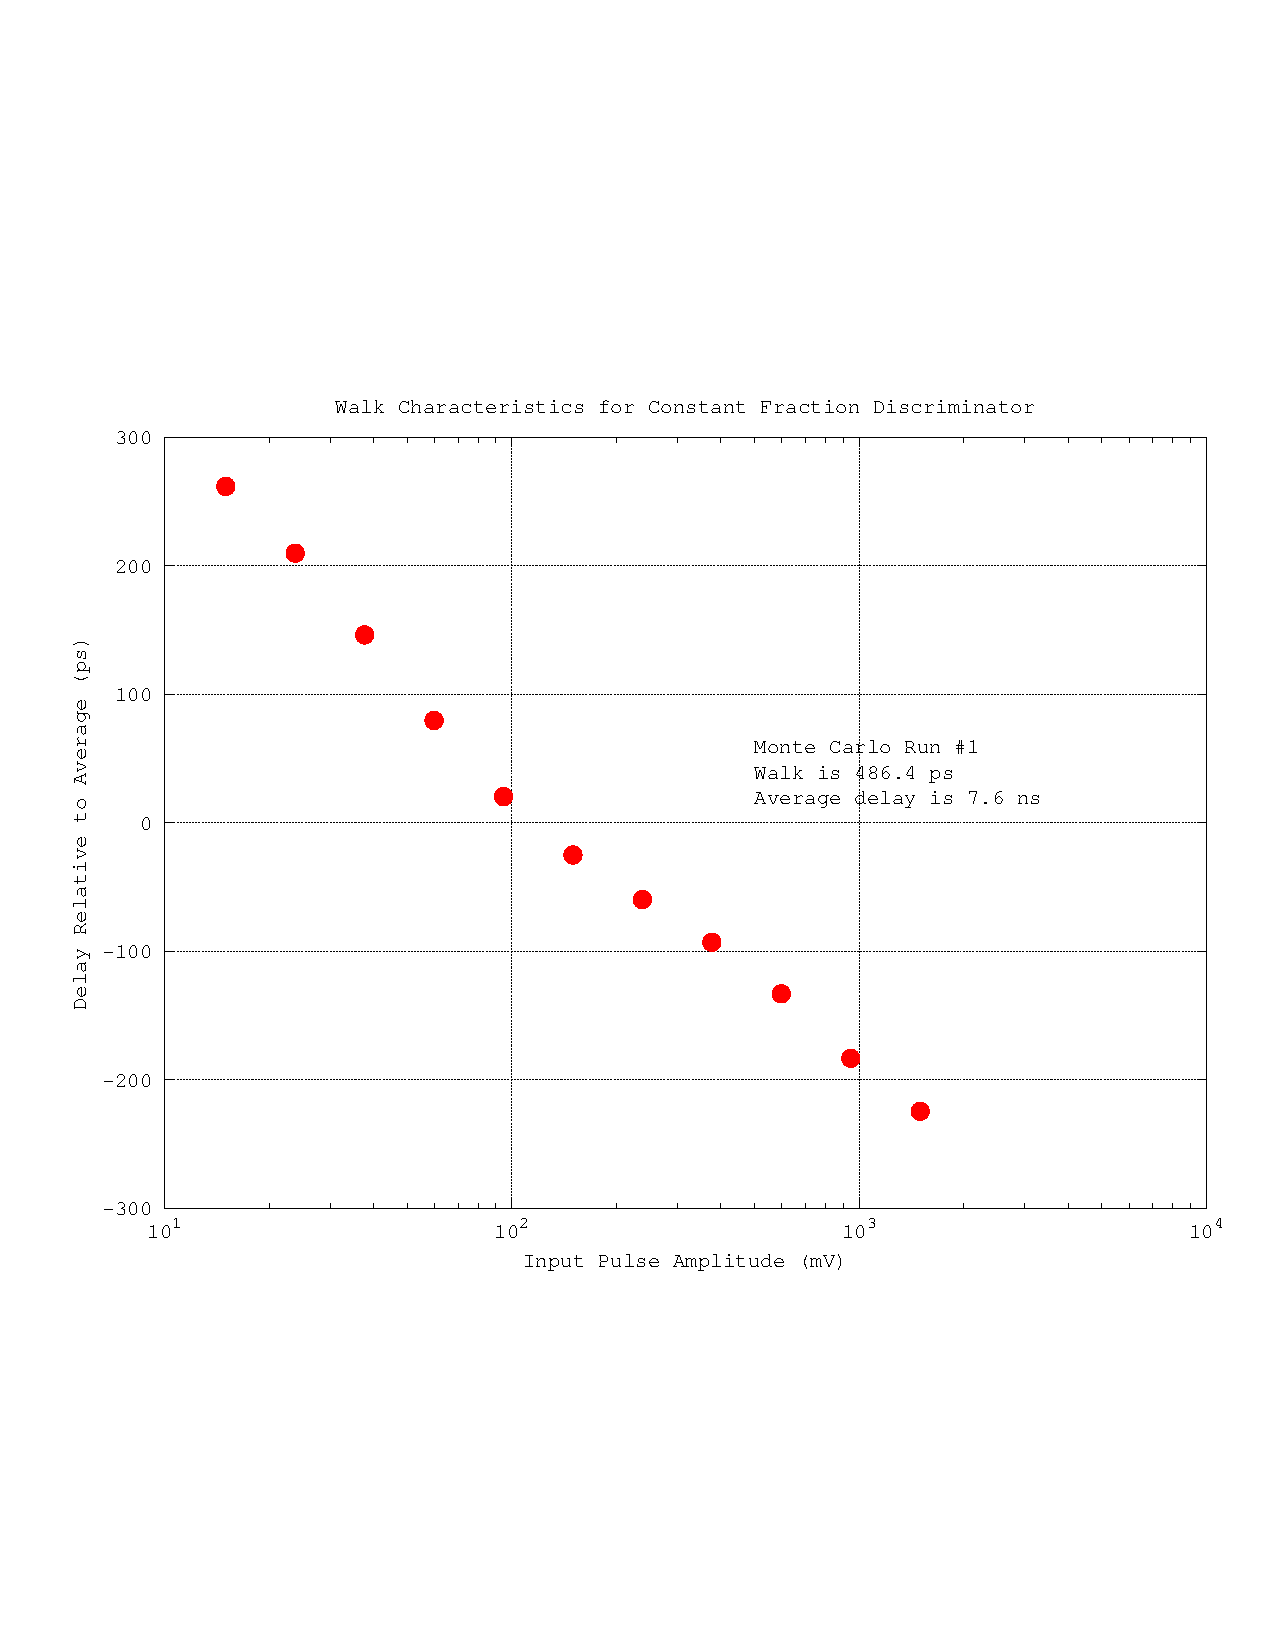
\includegraphics[scale=0.85,keepaspectratio=true]{./images/typical_walk.pdf} 	
 	\caption{Typical walk performance with a a signal whose rise time constant is 3 ns.}
 	\label{FIG:TYPICAL_WALK}
\end{figure}

\begin{figure}[htbp!]
	\centering
 	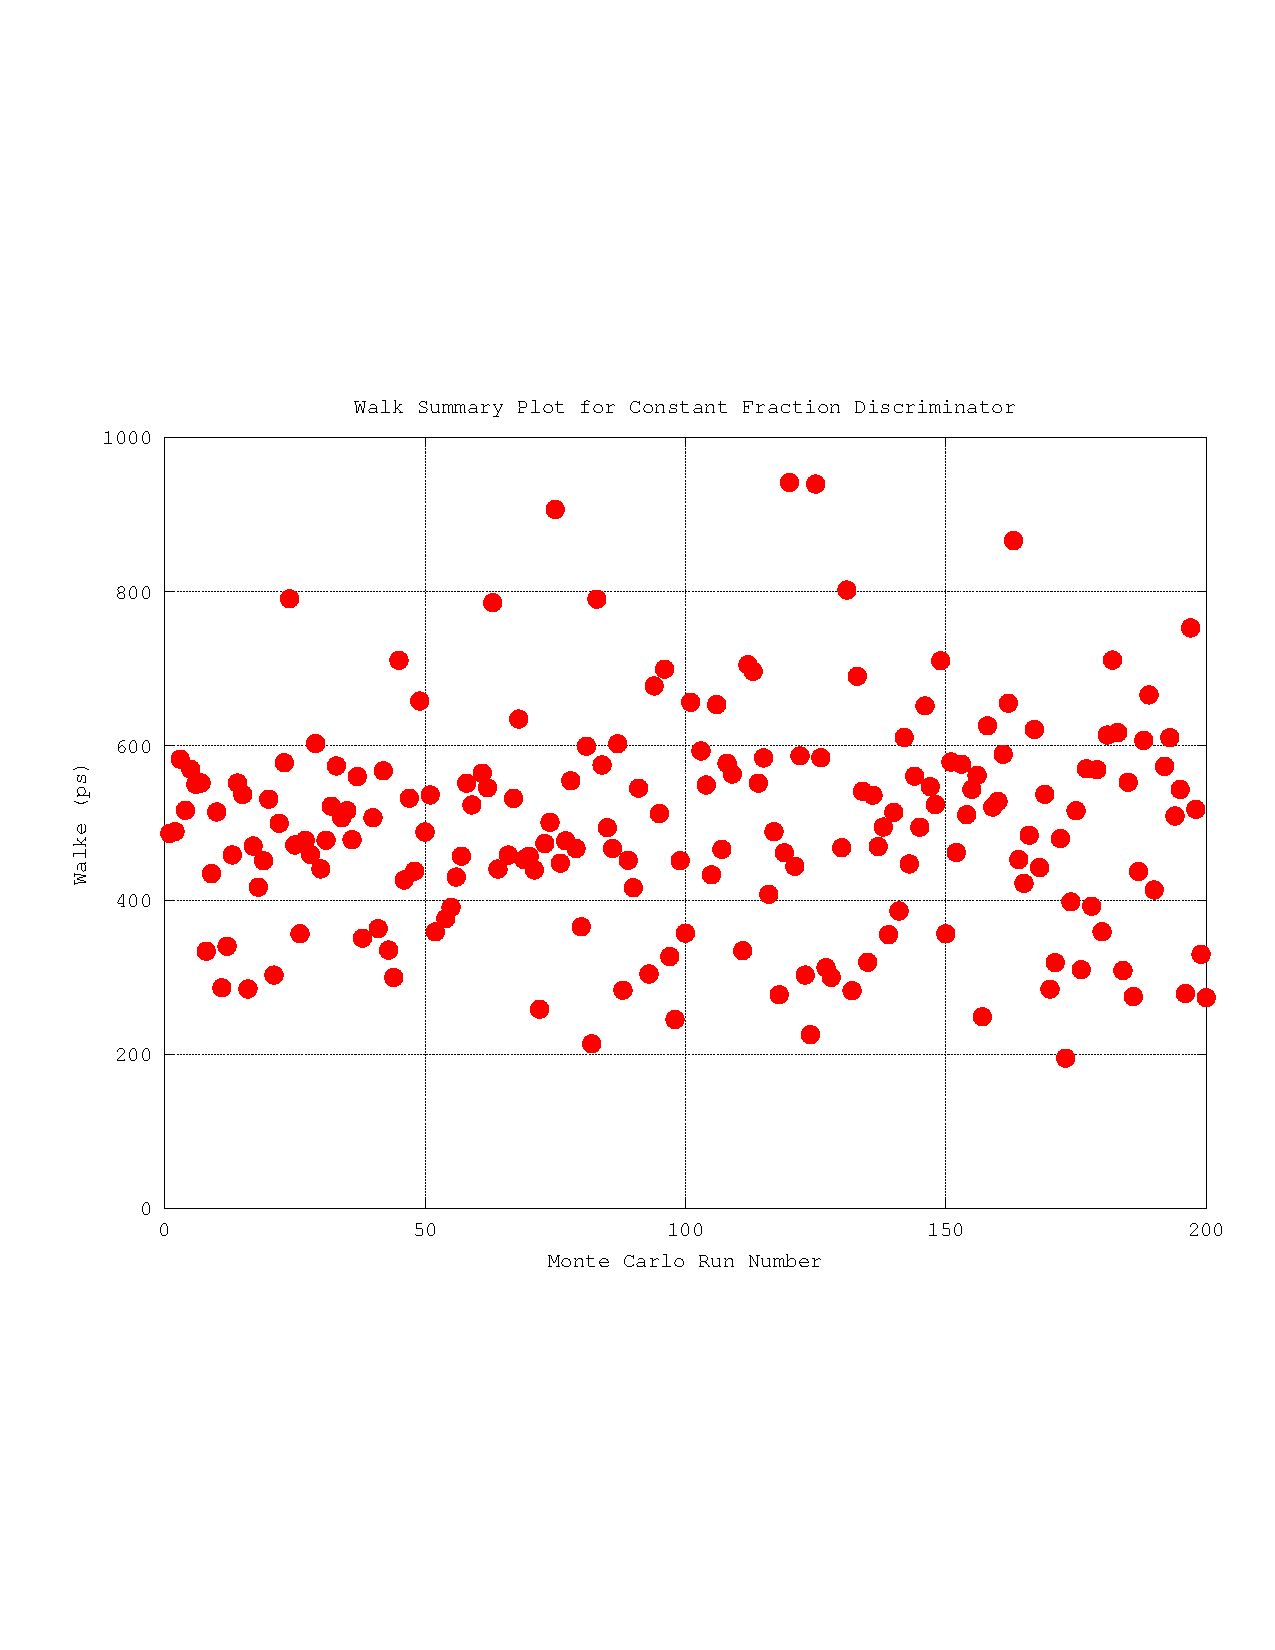
\includegraphics[scale=0.85,keepaspectratio=true]{./images/summary_walk.pdf} 	
 	\caption{Summary walk performance with a signal whose rise time constant is 3 ns.}
 	\label{FIG:SUMMARY_WALK}
\end{figure}
\section*{Design of Zero-Cross Circuit}


The purpose of the zero cross detector is to produce a digital signal which marks the onset of the analog input pulse. It is important that this time be independent of pulse amplitude, $A$.  The zero-cross circuit is constructed by cascading N differential amplifier stages (where we have chosen N equal to 5) each possessing a very wide bandwidth, but relatively low-gain ($\approx$ 4.5) with the final output stage driving a simple, yet very fast analog comparator.\\  


The purpose of cascading a relatively large number of high-bandwidth but low-gain stages is to force linear operation where delay is independent of amplitude. In short, the cascaded amplifier, which we shall refer to as the "pre-amplifier" serves as a slew rate enhancer.  For a first-order system, it is well-known that if the input risetime is not to be severely degraded, the bandwidth, BW, of the amplifier must obey the following equation\\

\begin{equation}
BW > \frac{0.35}{t_{10-90}} \approx \text{80 MHz}
\end{equation}


In the equation above we have assumed the shortest risetime constant that we must accommodate, \emph{i.e.}  2 $ns$. Since we are cascading N (here N is 5) stages, the BW of each stage must be increased by $\sqrt{N} \approx 2.2$ resulting in a differential amplifier bandwidth of 180 MHz if the overall BW is to be at least 80 MHz.  If the stage gain, G, is approximately 4.5, then the GBW of a single differential amplifier stage must exceed 800 MHz. The overall gain of the pre-ampifier is \\

\begin{equation}
Gain = G^N = 4.5^5 \approx \text{ 2000 or 66 dB}.
\end{equation}

Thus, the highest rate of change at the output of the pre-amplifier is approximately 2000 times larger than the input worst case rate of 1.8 $\frac{V}{\mu s}$.  Hence, the slew rate of the differential amplifier must be at least 3.6 $\frac{V}{ns}$ if the pre-amplifier is to be linear for signals near the zero-crossing point. In other words, CFD walk performance will be limited by how large a slew rate for the differentail amplifier can be achieved. Increasing the effective voltage of the input devices maximizes slew rate but how large of an effective voltage that can be used is ultimately limited by the supply voltage.\\


The theoretically predicted jitter performance plot for the short range mode is given in Figure~\ref{FIG:JITTER_FAST} and the expected performance in the long range mode is provided in Figure~\ref{FIG:JITTER_SLOW}.\\

\begin{figure}[htbp!]
	\centering
 	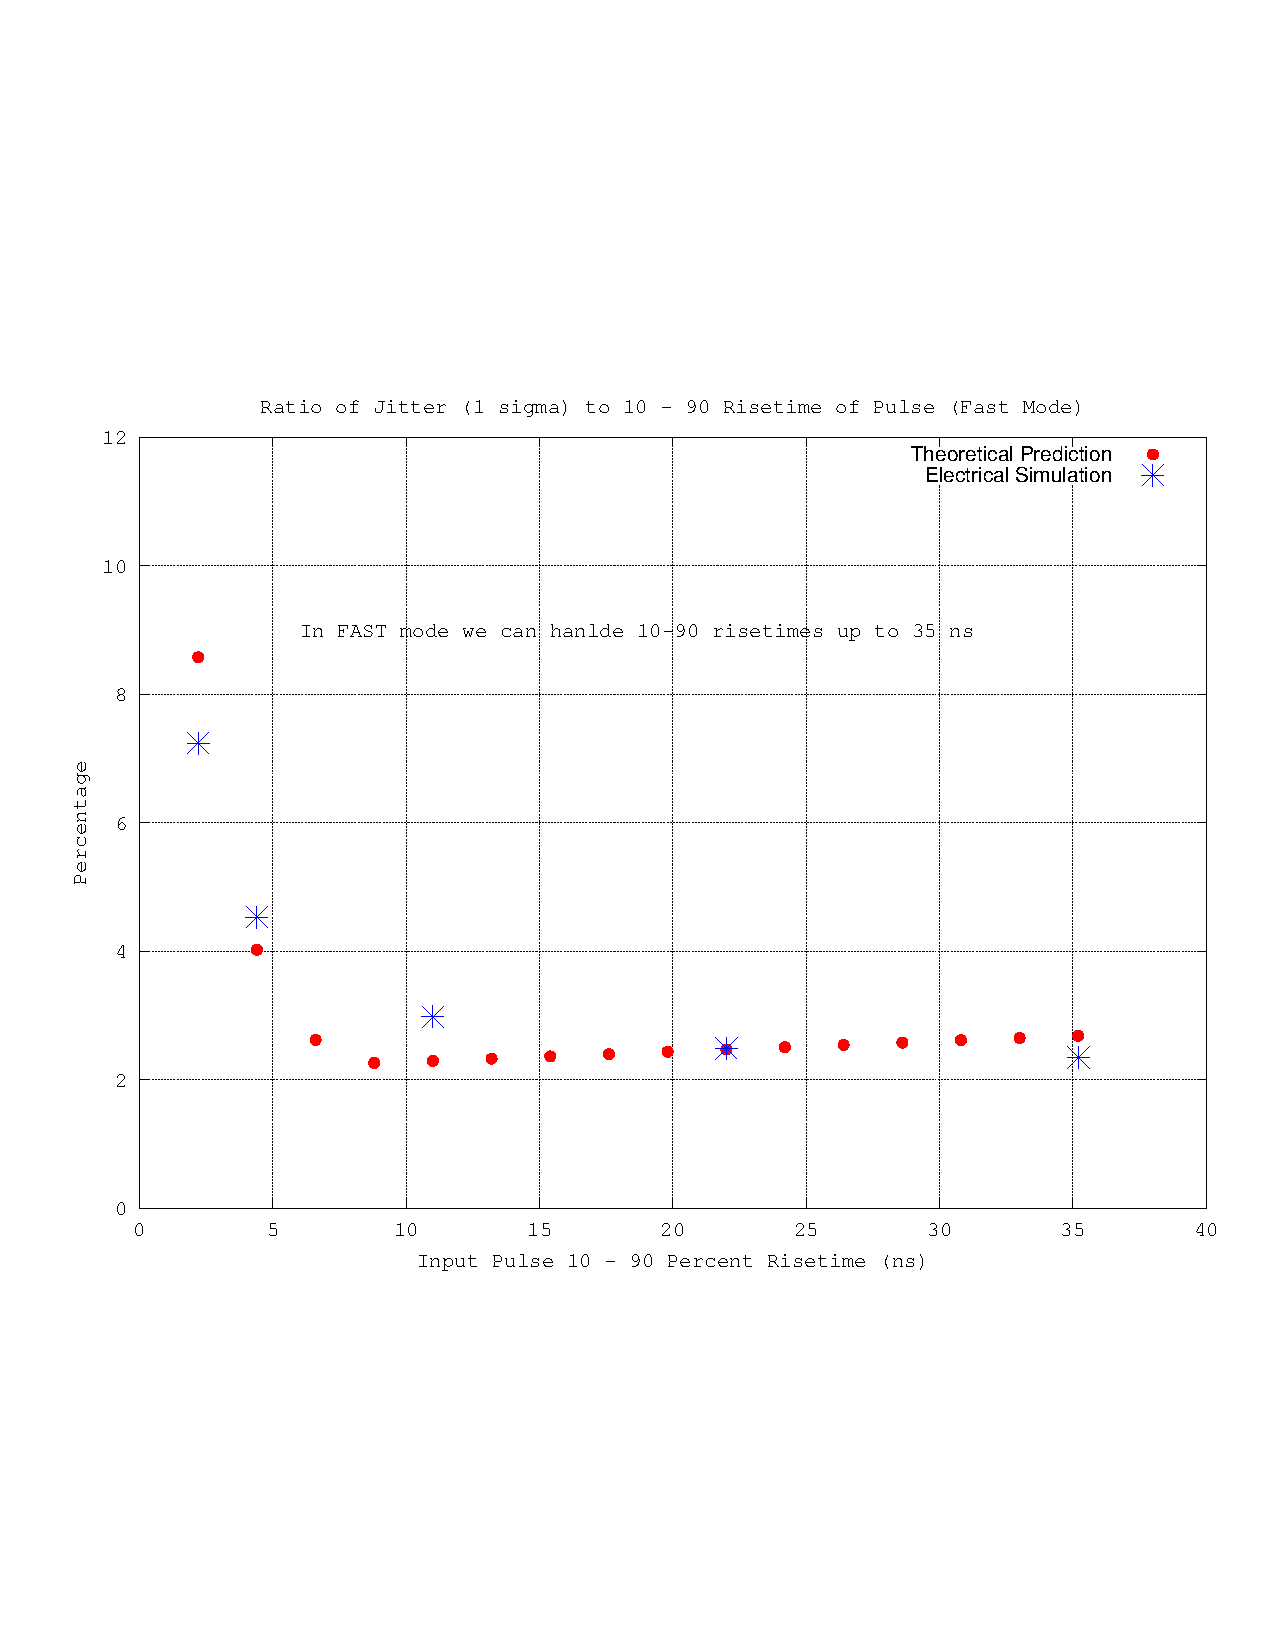
\includegraphics[scale=0.7,keepaspectratio=true]{./images/jitter_fast_mode.pdf} 	
 	\caption{Jitter performance for short time constant mode.}
 	\label{FIG:JITTER_FAST}
 	
\end{figure}

\begin{figure}[htbp!]
	\centering
 	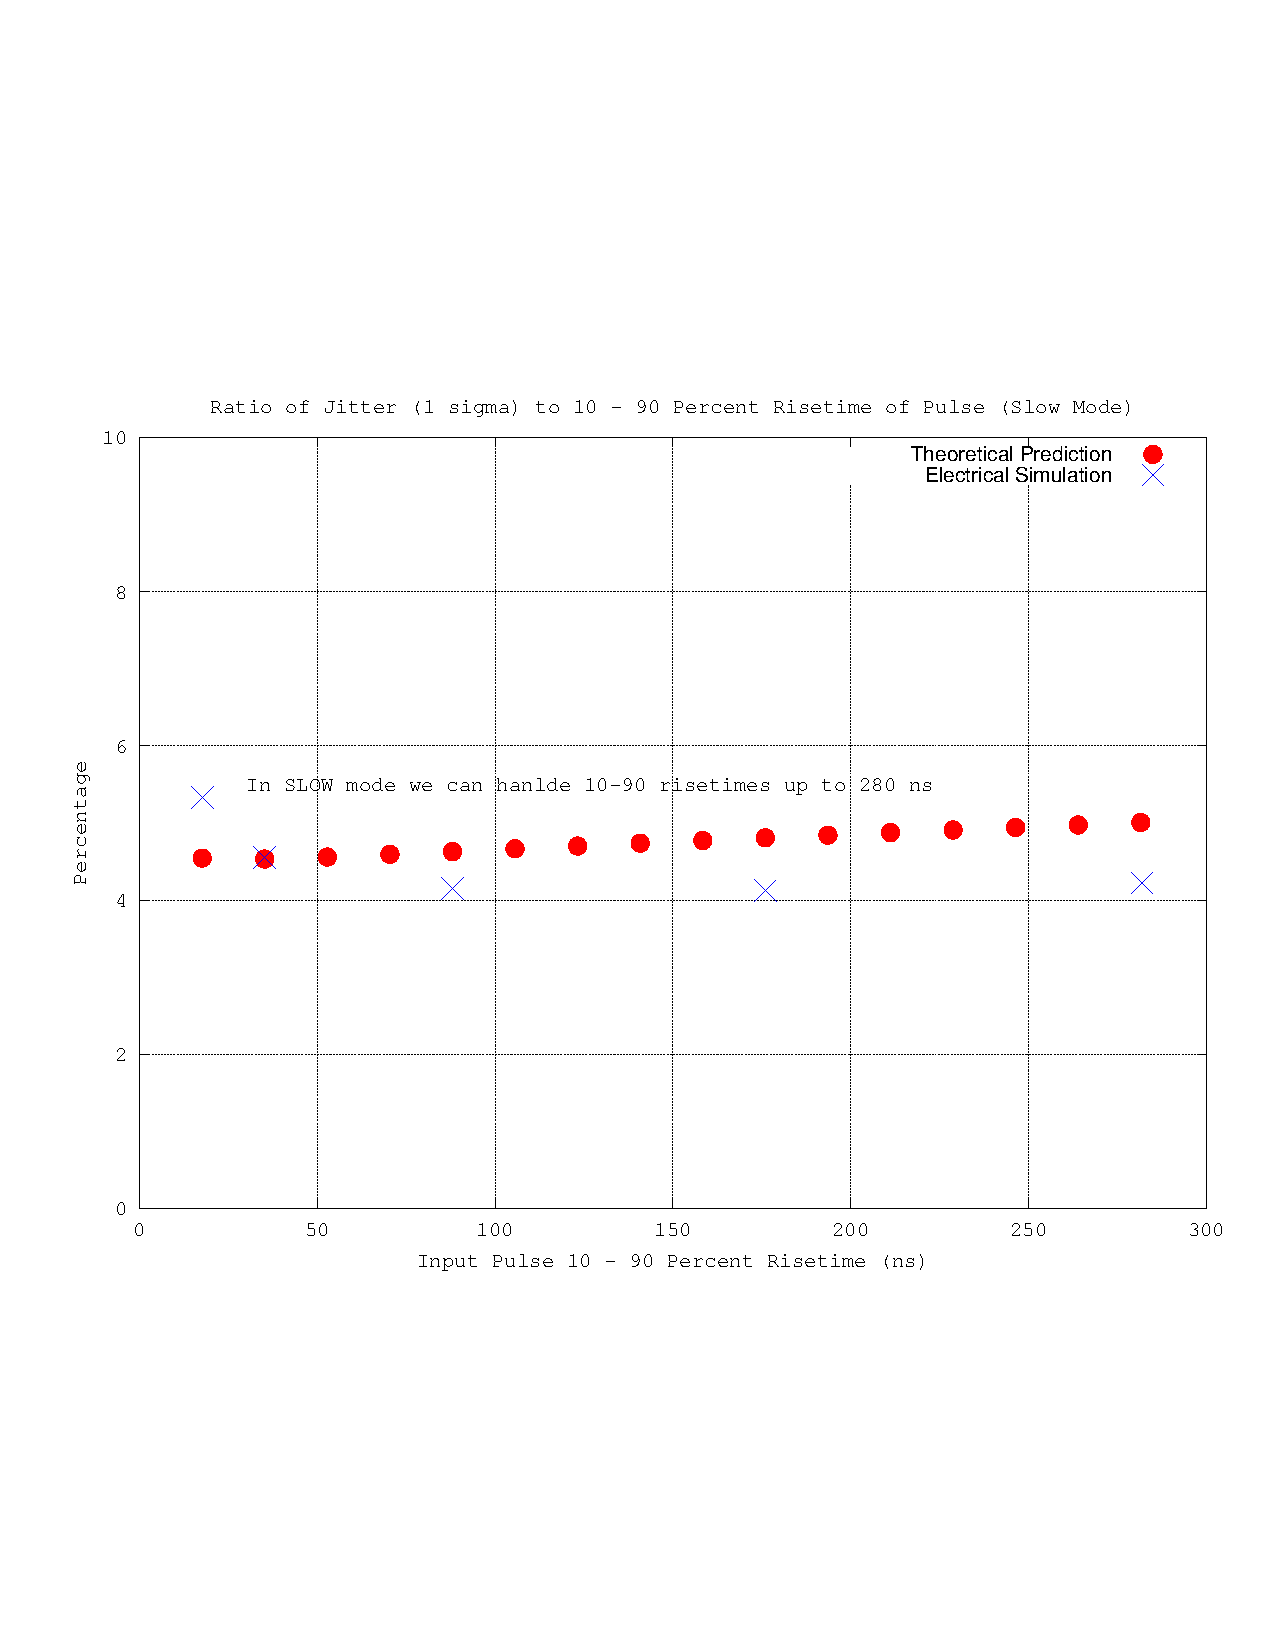
\includegraphics[scale=0.7,keepaspectratio=true]{./images/jitter_slow_mode.pdf}
 	\caption{Jitter performance for short time constant mode.}
 	\label{FIG:JITTER_SLOW}
\end{figure}


\subsection*{Design of Zero-Cross Differential Amplifier}


We will now describe the design of the wide-bandwidth, low-gain differential amplifier specified in the previous section. The amplifier is presented in Figure~\ref{FIG:ZC_DM_AMP}. \\

\begin{figure}[htbp!]
	\centering
 	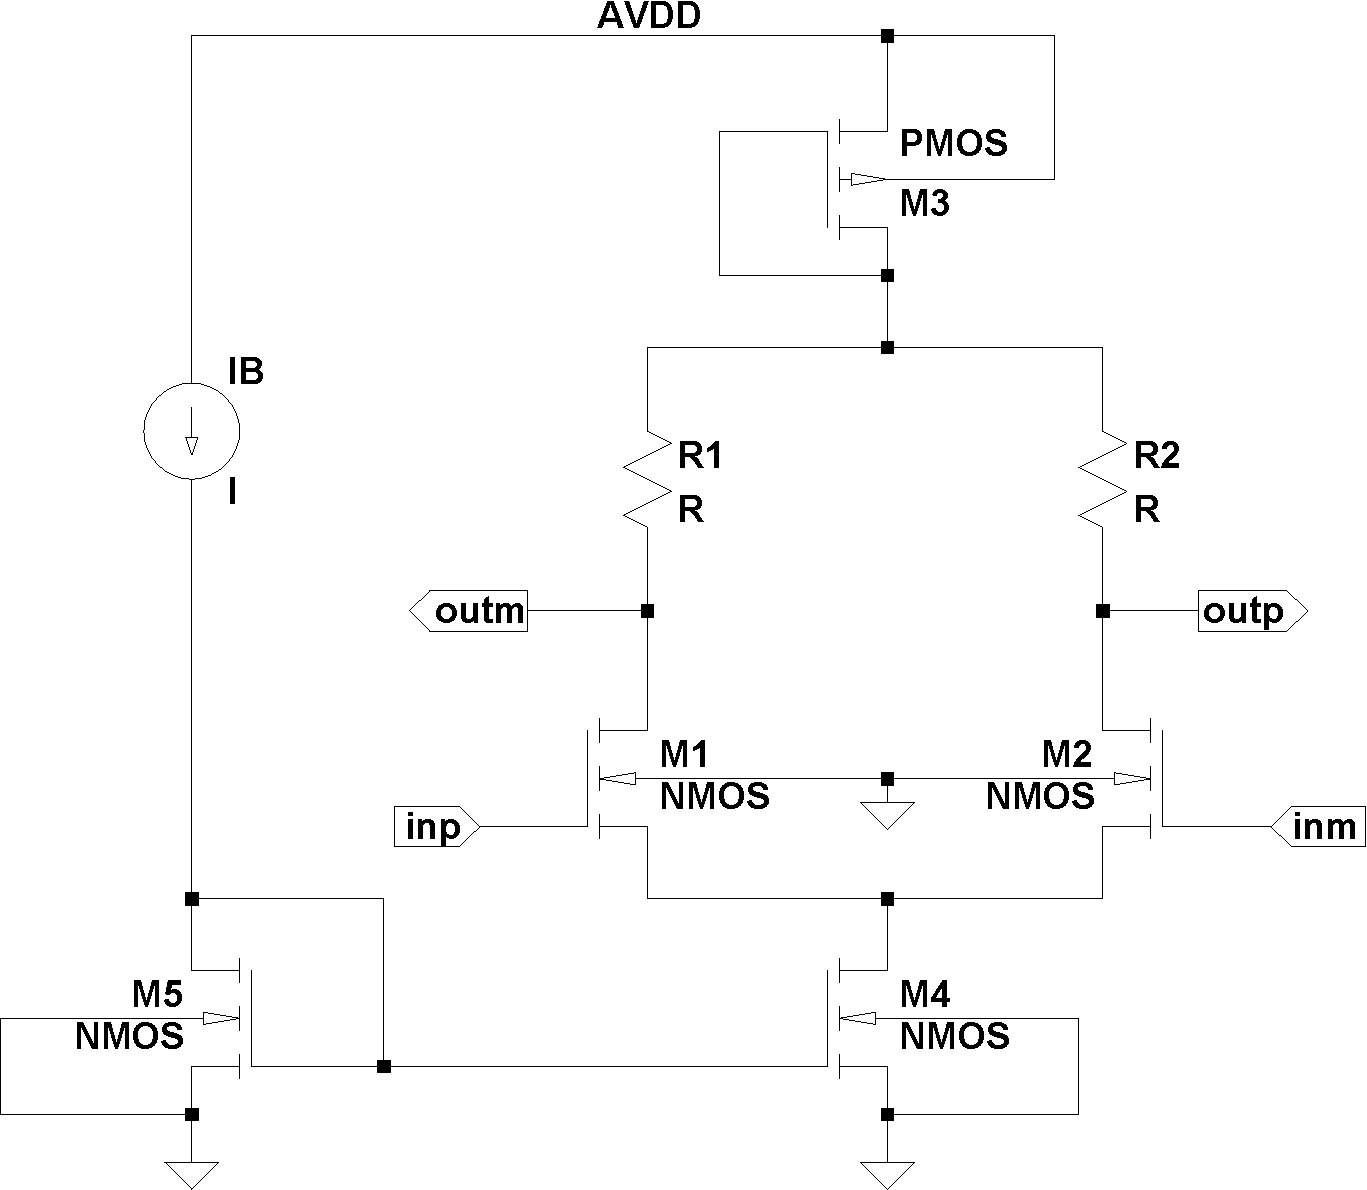
\includegraphics[scale=0.5,keepaspectratio=true]{./images/zc_dm_amp.pdf}
 	
 	\caption{Schematic of low-gain high-bandwidth differential amplfier.}
 	\label{FIG:ZC_DM_AMP}
 	
\end{figure}
 

Device sizes and bias currents are given in Table~\ref{TBL:ZC_DM_AMP}. The value of \emph{ng} represents the number of fingers (\emph{i.e.} gates) to use in the layout.\\ 


\begin{table} [htbp!]
\begin{center}
\begin{tabular}{|c|c|c|c|c|c|c|}
\hline 
 & W ($\mu m$) & L ($\mu m$) & ng & $I_B$ ($\mu A$) & $g_m$ ($\mu \mho$) & $V_{EFF}$ (mV)\\ 
\hline 
$M_1$ & 16.0 & 0.7 & 2 & 23 & 312 & 147 \\ 
\hline 
$M_2$ & 16.0 & 0.7 & 2 & 23 & 312 & 147 \\ 
\hline 
$M_3$ & 2.0 & 0.7 & 1 & 23 & 81.1 & 568 \\ 
\hline 
$M_4$ & 2.0 & 0.7 & 1 & 23 & 81.1 & 568 \\ 
\hline 
$M_5$ & 16.0 & 4.0 & 4 & 46 & 219 & 420 \\ 
\hline 
\end{tabular} 
\end{center}

\caption{Device Sizes for Zero-Cross Detector Differential Amplifier}
\label{TBL:ZC_DM_AMP}

\end{table}


The value of the resistors, $R_1$ and $R_2$, is 17 k$\Omega$ and the pair of matched resistors are implemented using a high resistance poly 2 layer. Transistor $M_3$ was added so that the output commmon-voltage could be set to approximately $\frac{V_{DD}}{2}$). Note, the current flowing through transistor $M_3$ is the same as the current, $I_B$, flowing through transistor $M_4$. Hence the drain of $M_3$ is a virtual ground in much the same main that the drain of $M_4$ is a virtual ground. Hence,the addition of $M_3$ has no impact on the speed of the amplifier. The low-frequency gain of stage is \\

\begin{equation}
A_0 = g_{m1} \cdot R \approx 4.6
\end{equation}


and the bandwidth of the stage is \\

\begin{equation}
BW = \frac{1}{2 \cdot \pi \cdot R \cdot C_L}
\end{equation}


where $C_L$ is the total capacitive load on the output node. \\


The output swing for the differential amplifer is $ 2 \cdot R \cdot I_B$, centered around $\frac{V_{DD}}{2}$, where $I_B$ is the tail current or 46 $\mu A$.  Transistor $M_5$ mirrors the PTAT primary current of 11.5 $\mu A$ and hence the value of 4 for the "ng" parameter is Table~\ref{TBL:ZC_DM_AMP}.\\

\subsection*{Design of Zero-Cross Comparator}


The comparator used in the zero-cross circuit is presented in Figure~\ref{FIG:ZC_CMP)}. Transitors $M_1$ - $M_4$ make up a simple symmetric Miller OTA. The input common-mode voltage is assumed to be approximately half the supply voltage. The DC bias current through each of the 4 transistors is approximately 200 $\mu A$.  The resulting GBW exceeds 3 GHz while the low-frequency open-loop gain is 26 dB.  \\

\begin{figure}[htbp!]
	\centering
 	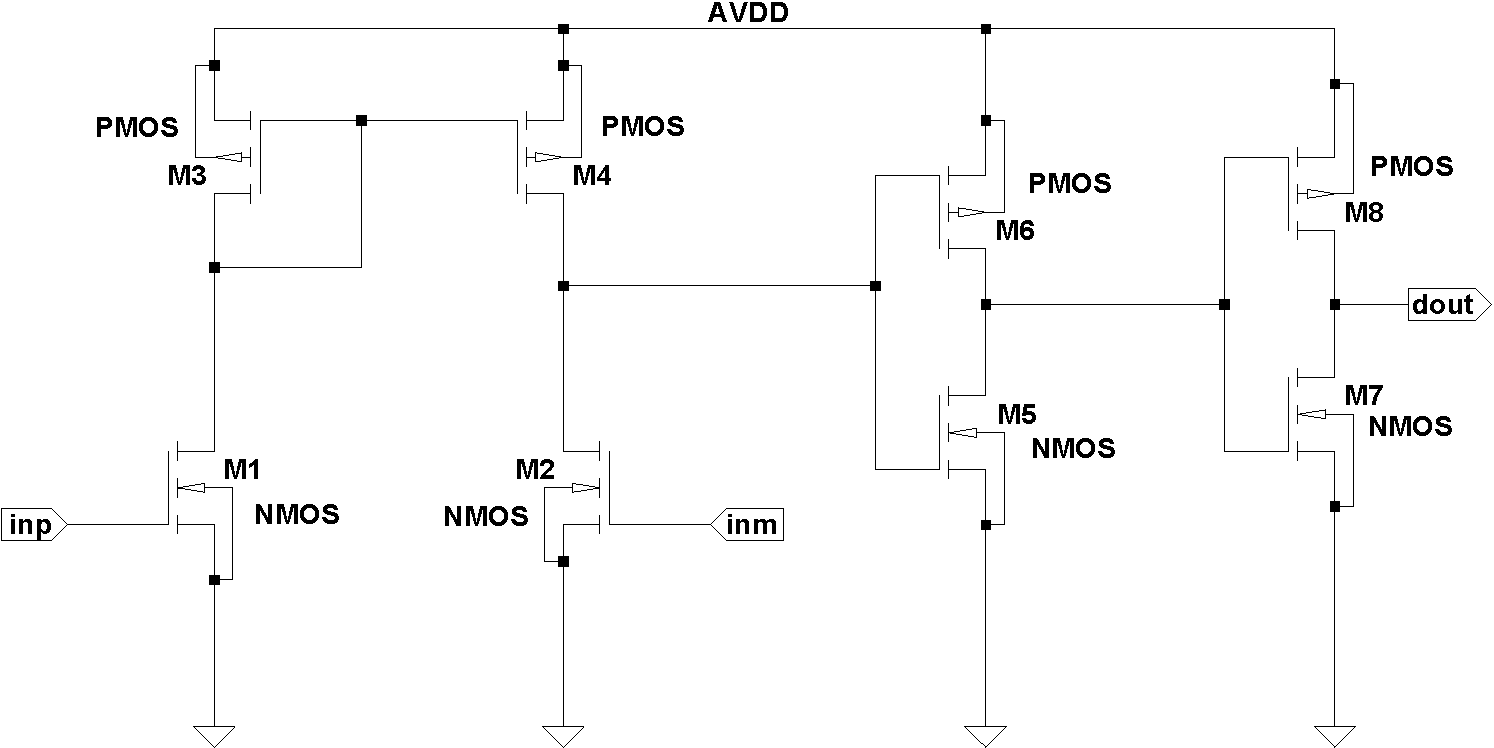
\includegraphics[scale=0.6,keepaspectratio=true]{./images/zc_cmp.pdf}
 	\caption{Schematic of high-bandwidth, very fast comparator.}
 	\label{FIG:ZC_CMP}
\end{figure}



Device sizes and bias currents are given in Table~\ref{TBL:ZC_CMP}. The value of \emph{ng} represents the number of fingers (\emph{i.e.} gates) to use in the layout.\\ 


\begin{table} [htbp!]
\begin{center}
\begin{tabular}{|c|c|c|c|c|c|c|}
\hline 
 & W ($\mu m$) & L ($\mu m$) & ng & $I_B$ ($\mu A$) & $g_m$ ($\mu \mho$) & $V_{EFF}$ (mV)\\ 
\hline 
$M_1$ & 16.0 & 0.7 & 2 & 23 & 312 & 147 \\ 
\hline 
$M_2$ & 16.0 & 0.7 & 2 & 23 & 312 & 147 \\ 
\hline 
$M_3$ & 2.0 & 0.7 & 1 & 23 & 81.1 & 568 \\ 
\hline 
$M_4$ & 2.0 & 0.7 & 1 & 23 & 81.1 & 568 \\ 
\hline 
$M_5$ & 16.0 & 4.0 & 4 & 46 & 219 & 420 \\ 
\hline 
\end{tabular} 
\end{center}
\caption{Device Sizes for Zero-Cross Comparator}
\label{TBL:ZC_CMP}
\end{table}


\subsection*{Dynamic Offset Cancelation Loop}


Offset of the zero-cross preamplfier is achieved by placing a very slow ampfifier in the feedback path.  For the purposes of this amplifier we will model the forward path using a single pole model.\\

\begin{equation}
A(s) = \frac{K_1}{1 + \frac{s}{\omega_1}}
\end{equation}


We will do the same for the slow amplifier in the feedback path.\\

\begin{equation}
B(s) = \frac{K_2}{1 + \frac{s}{\omega_2}}
\end{equation}


The closed-loop response is then given by \\

\begin{equation}
A_f(s) = \frac{A(s)}{1 + A(s) \cdot B(s)} 
\end{equation}


Using the expressions for A(s) and B(s) given above and assuming $K = K_1 \cdot K_2$ is large, then the closed-loop gain is approximately given by the expression \\

\begin{equation}
A_f(s) \approx \frac{1}{K_2} \cdot \frac{1 + \frac{s}{\omega_2}}{1 + \frac{s}{K \cdot \omega_2} + \frac{s^2}{K \cdot \omega_1 \cdot \omega_2}}.
\end{equation}\\


In the given application, we will choose $\omega_2 \gg \omega_1$.  Under this assumption, the lower and upper corner frequencies, $\omega_L$ and $\omega_H$, become \\

\begin{equation}
\omega_L \approx K \cdot \omega_2 \text{ and } \omega_H \approx  \omega_1
\end{equation}\\


One observes that since K is large, the value of $\omega_2$ must be at an extremely low frequency if $f_L$ is to be less than 10 $kHz$.\\


\subsection*{Design of Low Bandwidth, Low-Gain OTA}


As explained in the previous section, the amplifier in the feedback path used to dynamically offset compensate the  zero-cross pre-amplifier must posses a relatively low gain and a very small bandwidth.  Since the amplifier only needs to drive a resistive load, a Symmetric Miller OTA (Operational Transconductance Amplfier) was utilized.  The circuit is given in Figure~\ref{FIG:SMALL_GM_OTA}.


\begin{figure}[htbp!]
	\centering
 	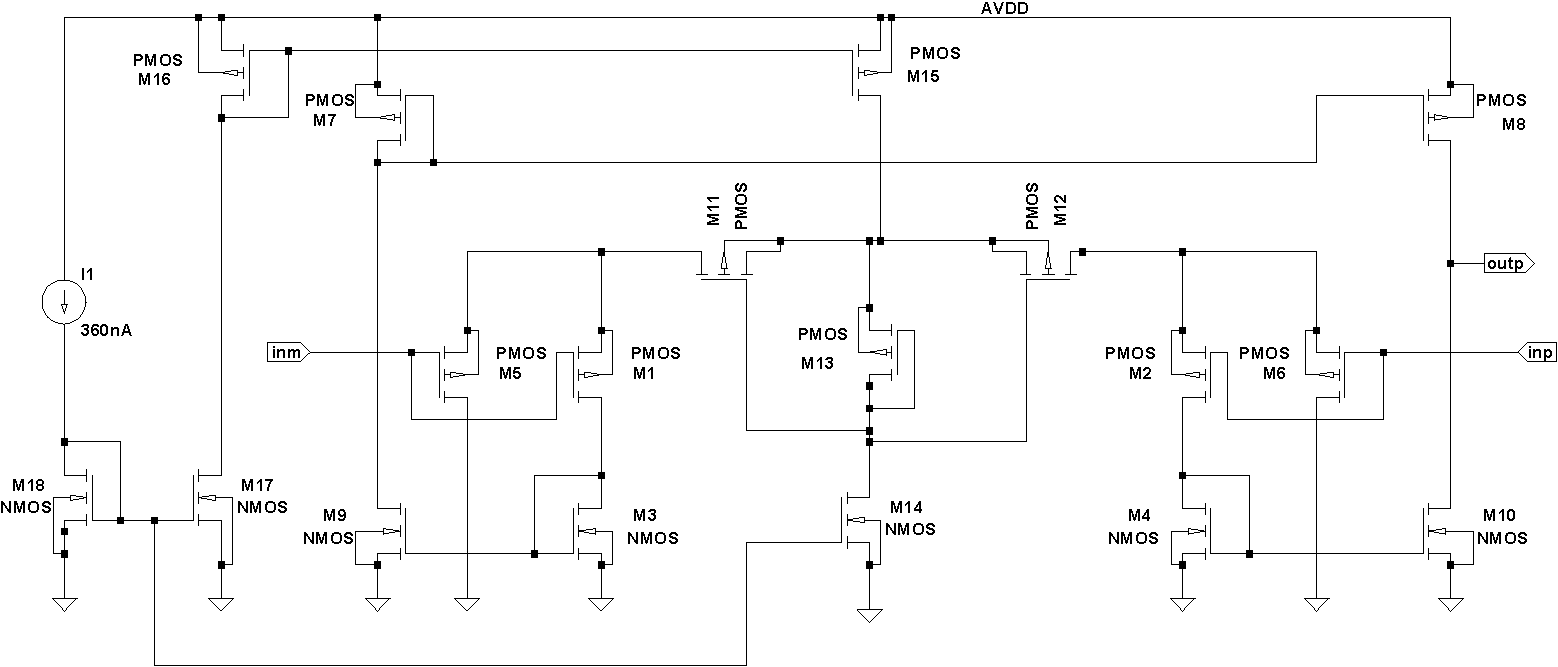
\includegraphics[scale=0.8,keepaspectratio=true, angle=90]{./images/small_gm_ota.pdf}
 	\caption{Schematic of low bandwidth, low gain OTA.}
 	\label{FIG:SMALL_GM_OTA}
\end{figure}


\section*{Design of Leading Edge Circuit}


The leading edge circuit is very very similar to the zero cross circuit.  

\subsection*{Design of Differential-to-Single Ended Converter}


The differential output voltage from the leading-edge preamplfier must be converted to a single ended current. This is done using the linear transconductor shown in Figure~\ref{FIG:LE_GM}.  The transconductance of the stage is $\frac{1}{R}$ where $R$ is 17 k$\Omega$.

\begin{figure}[htbp!]
	\centering
 	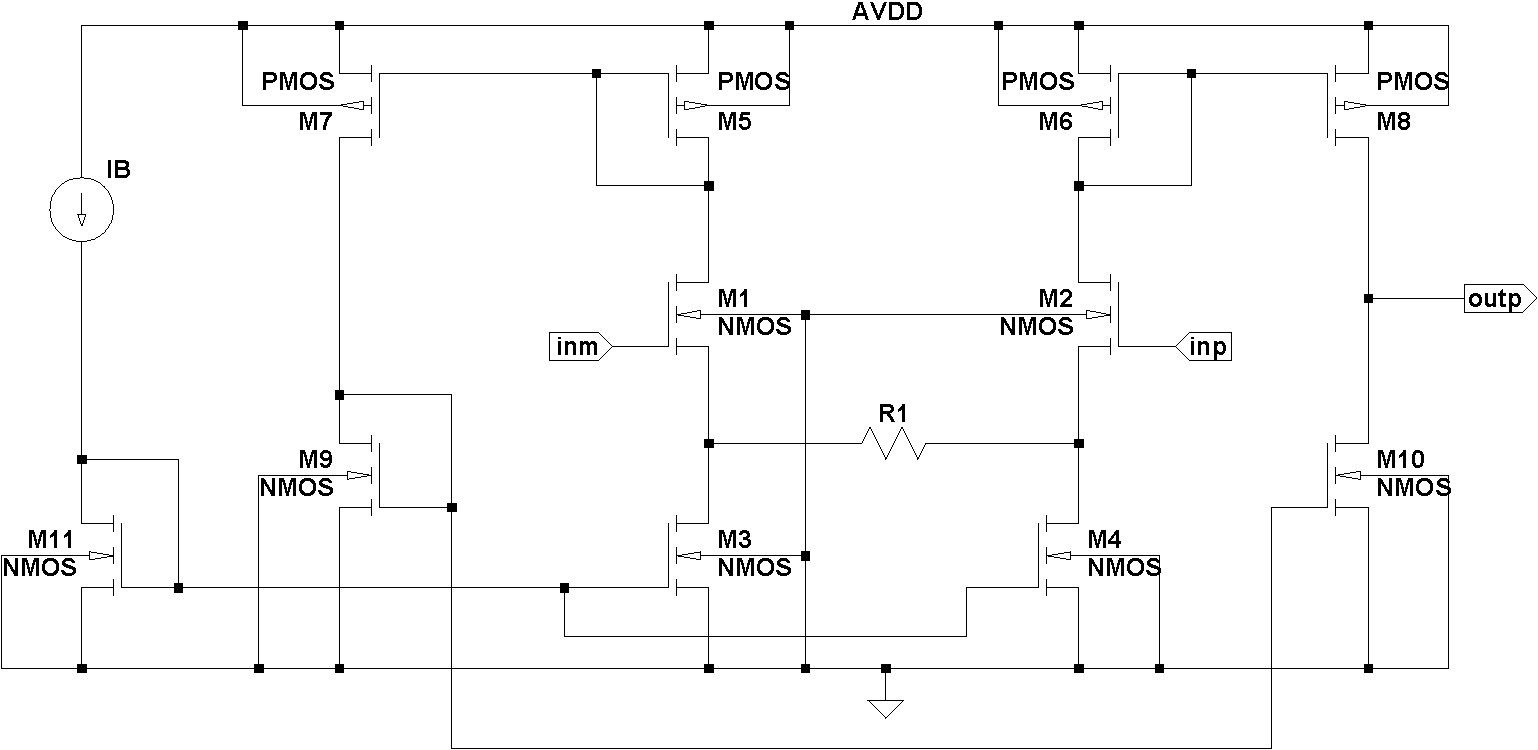
\includegraphics[scale=0.65,keepaspectratio=true]{./images/le_gm.pdf}
 	\caption{Schematic of differential voltage to single-ended current converter.}
 	\label{FIG:LE_GN}
\end{figure}


\subsection*{Design of Leading-Edge Comparator}

The leading-edge comparator is presented in Figure~\ref{FIG:LE_CMP}. It is very similar to the zero-cross comparator except two resistive voltage dividers have been added, one on the inverting and one on the non-inverting inputs.  All resisistors are 34 $k \Omega$ so that each divider can be represented by a Thevenin voltage equal to one-half the supply voltage and a Thevenin resistance of 17 $k \Omega$.  The divider on the non-inverting input is used to convert the sum of the diffential current output from the preamplfier and the current output of the DAC into a voltage which is then compared to $\frac{V_{DD}}{2}$.

\begin{figure}[htbp!]
	\centering
 	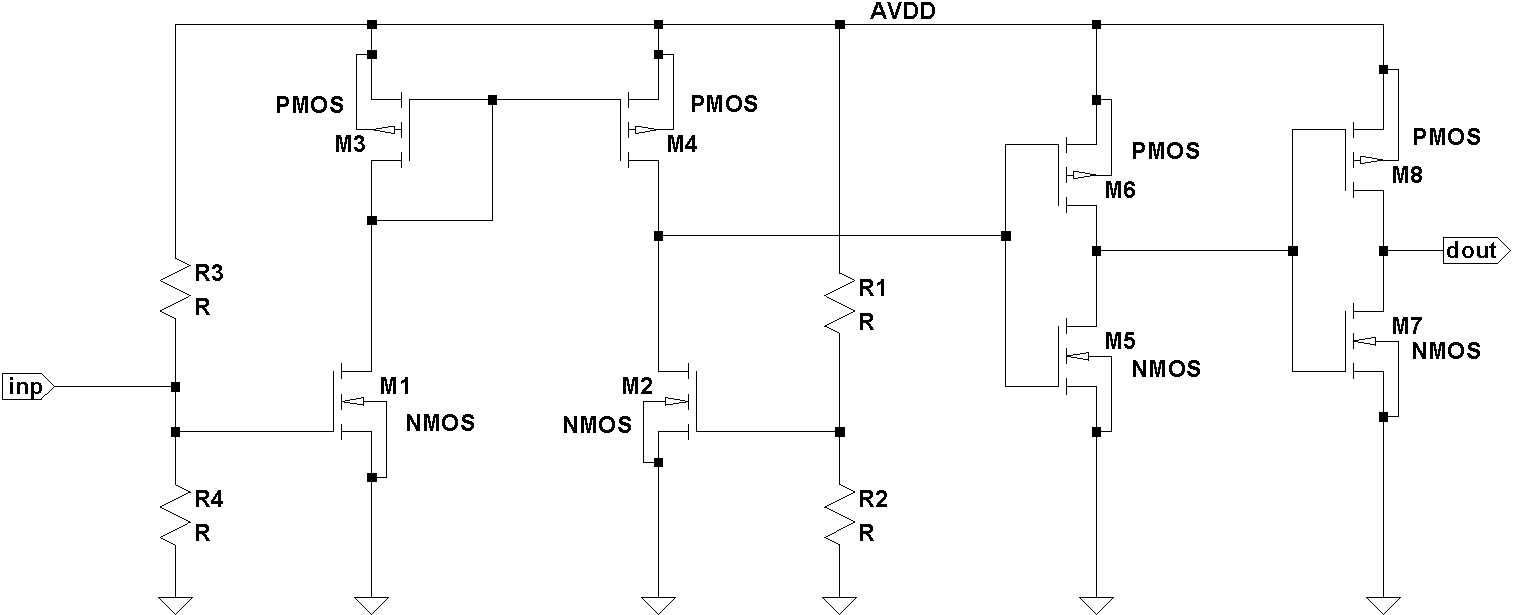
\includegraphics[scale=0.65,keepaspectratio=true]{./images/le_cmp.pdf}
 	\caption{Schematic of leading edge comparator.}
 	\label{FIG:LE_CMP}
\end{figure}


\subsection*{Design of Threshold Current DAC}


\end{document}